\documentclass[11pt]{article}
\usepackage{fullpage,amsmath, graphicx, epstopdf, tikz, amssymb}
\usepackage[linesnumbered,ruled,vlined]{algorithm2e}
\usetikzlibrary{arrows}
\usepackage{amsthm}
\usepackage{todonotes}
\renewcommand{\baselinestretch}{1.02}
\newcommand{\Q}[1]{\medskip\item {[{\em #1 marks\/}]}\ }
\usepackage{xcolor}
\newif\ifsol
\soltrue
\newcommand{\solution}[1]{{\ifsol \color{red} {#1} \fi}}

\newtheorem{claim}{Claim}

\newcommand{\down}[1]{\left\lfloor #1\right\rfloor}
\newcommand{\up}[1]{\left\lceil #1\right\rceil}

\begin{document}

\hfill CS 341, Spring 2020\par
\hfill Semih Salihoglu

\bigskip
\begin{center}\large\bf Assignment 6 (due Friday, July 31st, midnight EST)
\end{center}

\noindent{\bf Instructions:}
\begin{itemize}
\item Hand in your assignment using Crowdmark. Detailed instructions are on the course website.
\item Give complete legible solutions to all questions.
\item Your answers will be marked for clarity as well as correctness.
\item For any algorithm you present, you should justify its correctness
(if it is not obvious) and analyze the complexity.
\end{itemize}

\begin{enumerate}

\Q{25} {\em Programming Question:} This is a programming question. Details on how you will submit your code will be posted on Piazza.

Implement Bellman Ford's algorithm that takes in a directed graph $G(V, E)$ with arbitrary edge weights and a source node $s$ and outputs one of two things: (1) if there are no negative weight cycles in $G$, then the shortest distance from $s$ to every other node $v \in V$; or (2) if there is a negative weight cycle outputs ``ERROR: NEGATIVE WEIGHT CYCLE'' (without the quotations). There will be 25 test cases. 20 of these cases will test these two outputs. 

An additional 5 cases will contain inputs with negative weight cycles and we will ask you to output an actual negative weight cycle as part of the output after the ``ERROR: NEGATIVE WEIGHT CYCLE'' line. The actual negative weight cycle can be output as follows: keep track of the predecessors of nodes in a separate data structure as you find the shortest paths from $s$. Then, first detect that there is a negative weight cycle. Recall that this can be done by observing that at least one node's, say $v$'s, distance changes at the $n$'th iteration of the algorithm. Then follow the predecessors of $v$ iteratively until one of the predecessors, say node $w$ is repeated twice. The set of edges between $w$'s first and second appearance gives a negative weight cycle.

You can either use Python or C++. Your program should read from standard input and print to standard output. For each testcase, the first line of input will contain 3 (space-separated) integers $n, m, s$, where $n$ is the number of vertices of the input graph, $m$ the number of edges and $s\in\{0,\ldots ,n-1\}$ the source vertex. Then, $m$ lines will follow where each one also contains 3 (space-separated) integers $u, v, w$ that represent an edge from $u\in\{0,\ldots ,n-1\}$ to $v\in\{0,\ldots ,n-1\}$ with weight $w\in\mathbb{Z}$. The first line of your output should either contain $n$ (space-separated) integers $d_i$ that represent the shortest distance from $s$ to $i$ in the graph, or ``ERROR: NEGATIVE WEIGHT CYCLE''. For the source node $d_s=0$, and if $i$ is not reachable from $s$, then $d_i=\text{inf}$. For the last 5 marks, in the case of error, your program should also output a second line that contains a (space-separated) sequence of nodes which form a negative weight cycle. The first and last node muct be the same.

Input sample:\\
{\tt 5 6 0}\\
{\tt 0 1 2}\\
{\tt 0 2 -2}\\
{\tt 0 3 5}\\
{\tt 2 1 1}\\
{\tt 2 3 8}\\
{\tt 4 3 1}\\
Output sample:\\
{\tt 0 -1 -2 5 inf}

%You can output the negative weight cycle by keeping track of the predecessors (or successors) of nodes as you find the shortest paths. Then after you run Bellman Ford's algorithm for the extra $n$'th iteration to detect a cycle, if there is a negative weight cycle, one of the nodes

\newpage
\item{[{\bf Shortest Paths (13 marks)}]} 
\begin{itemize}

\item[(a)][3 marks] Recall that Dijkstra's algorithm does not work when the input graph have negative weighted edges. Consider the following fix to Dijkstra's algorithm: Given a graph $G(V, E)$ with possibly negative weighted edges, find the minimum weight edge $e=(u, v)$ in $G$ and add $|w(e)|$ to every edge in $G$. This constructs a new graph $G'$ that contains only non-negative edges. Now run Dijkstra's algorithm on $G'$. Construct a counter example to show that this fix will not correctly find the shortest paths in the original $G$.

\begin{center}\begin{figure}[h]
    \centering
    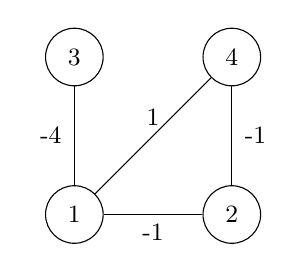
\begin{tikzpicture}
	\tikzset{text width={width("10")},
			align=center,
			font=\small}
	\tikzset{vertex/.style = {shape=circle,draw,minimum size=1em}}
	\tikzset{edge/.style = {-,> = latex'}}
    % vertices
    \node[vertex] (a) at  (0,0) {1};
    \node[vertex] (b) at  (2,0) {2};
    \node[vertex] (c) at  (0,2) {3};
    \node[vertex] (d) at  (2,2) {4};
    %edges
	\draw[edge] (a) to node[left] {-4} (c);
	\draw[edge] (a) to node[below] {-1} (b);
	\draw[edge] (b) to node[right] {-1} (d);
	\draw[edge] (d) to node[above] {1} (a);
\end{tikzpicture}
\caption{$G$}

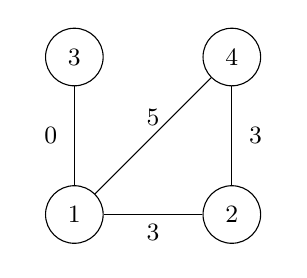
\begin{tikzpicture}
	\tikzset{text width={width("10")},
			align=center,
			font=\small}
	\tikzset{vertex/.style = {shape=circle,draw,minimum size=1em}}
	\tikzset{edge/.style = {-,> = latex'}}
    % vertices
    \node[vertex] (a) at  (0,0) {1};
    \node[vertex] (b) at  (2,0) {2};
    \node[vertex] (c) at  (0,2) {3};
    \node[vertex] (d) at  (2,2) {4};
    %edges
	\draw[edge] (a) to node[left] {0} (c);
	\draw[edge] (a) to node[below] {3} (b);
	\draw[edge] (b) to node[right] {3} (d);
    \draw[edge] (d) to node[above] {5} (a);
\end{tikzpicture}
\caption{$G'$}
\end{figure}\end{center}

If we run Dijkstra's algorithm on $G'$, the shortest path from vertex 1 to vertex 4 will be $\{(1, 4)\}$ 
in $G'$. But the shortest path from vertex 1 to vertex 4 is $\{(1, 2), (2, 4)\}$.

\newpage
\item[(b)] [5 marks] A {\em grid graph} is a graph in which the nodes can be placed on a grid such that there is an edge going from left to right between vertices and bottom to up. Specifically in an $r \times c$ grid graph, there are $r \times c$ vertices, labeled with $v_{ij}$, where $i=\{1,\ldots,r\}$ and $j=\{1,\ldots,c\}$. Visually $v_{11}$ is at the bottom left and $v_{rc}$ is at the top right corner of the grid and rows and columns are increasing in number from bottom to top and left to right, respectively. There is an edge between $(v_{ij},v_{i,(j+1)})$ (except from  vertices on the right most column) and $(v_{ij}, v_{i+1, j})$ (except from vertices on the top row vertices). Figure~\ref{fig:grid} shows an $3 \times 4$ grid graph.

\begin{figure}[h]
\centerline{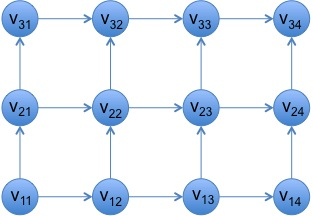
\includegraphics[height=4cm]{grid-graph.jpg}}
\caption{A $3 \times 4$ grid graph.}\label{fig:grid}
\end{figure}


Consider an $r \times c$ grid graph $G$ with arbitrary weights on the edges (i.e., weights can be negative). Show how to use Dijkstra's algorithm to find the shortest paths from $v_{11}$ to all other nodes in this graphs. Prove that your algorithm is correct. 

We can apply the process in part (a) frist and run Dijkstra's algorithm on $G'$.

\textbf{Proof of correctness:} Let a path from $V_{11}$ to $u$ in $G$ be $P$, $W(P)$ be the total weight of 
$P$ in $G$ and $W'(P)$ be the total weight of $P$ in $G'$. $W(P') = W(p) + |P| \cdot |w(e)|$, where $e$ is the minimum edge 
weight in $G$. Since for a grid graph, all the paths form $V_{11}$ to any $u$ have the same length. Hence for all 
paths form $V_{11}$ to any $u$, if $W(p_1) < W(p_2)$ in $G$, $W(p'_1) < W(p'_2)$ in $G'$. Hence we can convert each 
edge weight to non-negative but still return the correct answer.

\newpage
\item[(c)] [5 marks] Given an $r \times c$ grid graph $G$, describe an $O(cr)$ algorithm that finds the shortest paths from $v_{11}$ to all other nodes in the graph. Show how a slight modification of your algorithm can be use to also find the {\em longest paths} from $v_{11}$ to all other nodes (for the part about longest paths, you do not need to prove correctness, but just need to mention what the change is). An interesting fact is that the longest paths problem on general graphs is NP-complete.

\begin{algorithm}[h]
    \caption{ShortestPath($G(V, E), v_{11}$)}
    topologically sort $G$\\
    $SD[v_{11}] = (0, \emptyset)$\\
    $SD[v] = (\infty, \emptyset)$ for all $v \neq v_{11}$\\
    \For{$v \in G$ in topologically sorted order} {
        \For{$u \in inNbr(v)$} {
            $SD[v].first = min(SD[v], SD[u] + w(u, v))$\\
        }
        $SD[v].second = SD[v].second \cup \{ u \}$ where $u$ is in the shortest path to $v$\\
    } 
    \Return{$SD$}
\end{algorithm}

\textbf{Proof of Correctness:} By the way of how a grid graph is constructed, every grid graph does not have 
any cycle. Thus, for any vertex that is not $v_{11}$ in $G$, the shortest path from $v_{11}$ is the shortest 
path to its in-neighbours plus the weight of the edge between its in-neighbour and itself. For $v_{11}$, the 
shortest path is $0$.

\textbf{Runtime Analysis:} Since $|V(G)| = r \times c$, the number of horizontal edges is $r(c - 1)$ and 
the number of horizontal edges is $c(r - 1)$. Thus $|E(G)| = r(c - 1) + c(r - 1) = O(cr)$.\\
topologically sort $G$ takes $O(m + n) = O(cr)$. Since we loop over each vertex and each edge exactly once, 
the loop takes $O(cr + |E(G)|) = O(cr)$ times. So the total runtime is $O(cr)$.\\
If we want to find the longest path from $v_{11}$ to all other nodes, we just use $max$ instead of $min$ on 
line $6$ and append the vertex in the longest path in line $7$.

\end{itemize}

\newpage
\Q{15}
Suppose we have a set of directed and strongly connected graphs $G_1=(V, E_1),G_2= (V, E_2), \ldots, G_k=(V, E_k)$. Fix two nodes $s$ and $t$, and consider finding an $s$-$t$ path $P$, where the length of $P$ is the number of edges in $P$; that is, $\ell(P) = \sum_{e\in P} 1$. Our goal is to produce a sequence of paths $P_1, P_2, \ldots, P_k$ so that for each $i$, $P_i$ is an $s$-$t$ path in $G_i$, and such that its total cost below is minimized:
$$
cost(P_1, P_2, \ldots, P_k) = \sum_{i=1}^k \ell(P_i) + \lambda \sum_{j=1}^{k-1} \mathbf{1}(P_j\ne P_{j+1}),
$$
where $\mathbf{1}(P_j\ne P_{j+1}) = 1$ if the path $P_j$ is different from $P_{j+1}$ and $\mathbf{1}(P_j\ne P_{j+1}) = 0$ otherwise. Here $\lambda > 0$ is a given integer constant that is part of the problem specification and that balances the two conflicting goals: (1) minimizing the total lengths of the paths, and (2) minimizing the number of path switches.

\begin{enumerate}
	\Q{5} Suppose it is possible to choose a \emph{single} path $P$ that is an $s$-$t$ path in each of the $k$ graphs $G_1, \ldots, G_k$. Give an $O(k|V|^2)$ polynomial time algorithm to find the minimum cost (equivalently, \emph{shortest} since the second sum evaluates to zero) such path. Faster algorithms will get full credits as well.
	
	[\emph{Hint}: This path may or may not be the shortest $s$-$t$ path in any particular graph $G_i$ but you can construct a new graph to help solve the question.]
    
    Let $|V| = n$.
\begin{algorithm}[h]
    \caption{MinCostP($G_1, \dots, G_k$)}
    convert $E_1, \dots, E_k$ to adjacent matrices\\
    $E' = E_1$\\
    \For{$v \in V$} {
        \For{$i = 2, \dots, k$} {
            $E'[v] = E'[v] \cdot E_i[v]$\\
        }
    }
    use BFS on $G'(V, E')$ starting from $s$ and find the shortest s-t path.\\
    $p = BFS(G', s, t)$\\
    \If{$p = \emptyset$} {
        \Return{$(\emptyset, \infty)$}
    }
    \Return{$(p, |p|)$}
\end{algorithm}
    
\textbf{Proof of Correctness:} Clearly, $E'[u, v] = 1$ if and only if $E_1[u, v] = \cdots = E_k[u, v] = 1$.
so $G'$ is the graph $V(G') = V$ and $|E(G')| = E_1 \cap \dots \cap E_k$.
If a s-t path $P$ is in every graph, $P$ is in $G'$. Hence we can just us Dijkstra's algorithm to find a 
shortest s-t path in $G'$.\\
\textbf{Runtime Analysis:} If a graph $G$ is complete(every vertex has degree $n - 1$), $E(G) = \frac 
{n(n - 1)} {2}$. Hence $E_1 = \cdots = E_k = O(n^2)$. Since each convertion go through all edges exactly once. 
The convertion takes $O(k n^2)$ time. \\
Line 3 to 5 takes at most $O(kn^2)$ time(assuming multiplication takes $O(n)$ time). \\
Since BFS takes $O(n^2 + n) = O(n)$ time. The total runtime is 
$T(n) = O(kn^2) + O(n^2) = O(k |V|^2)$.

\newpage
	\Q{10} Give an $O(k^3|V|^2)$ polynomial time algorithm to find a sequence of paths $P_1, P_2, \ldots, P_k$ of minimum cost, where $P_i$ is an $s$-$t$ path in $G_i$ for $i=1,\ldots,k$. Argue correctness of your algorithm and analyze its run time complexity. You do not need to give pseudo-code for finding the actual paths but explain your algorithm clearly and succinctly. Faster algorithms will get full credits as well.
	
	[\emph{Hint}: use part (a) and dynamic programming. Two observations may be helpful here: (1) If we knew between which two graphs the \emph{last} switch of path occurred, then we can reduce the size of our problem; (2) once we specify the last switch to occur say between graph $G_i$ and $G_{i+1}$, then by inspecting the definition of the cost and with help in part (a) we can figure out which path we should choose from graph $G_{i+1}$ onwards.]
    
    \begin{algorithm}[h]
        \caption{MinCost($G_1, \dots, G_k$)}
        $C_{k \times k}$ where $C[i][j] = \infty$ for all $i, j$\\
        \For{$i = 1, \dots, k$}{
            \For{$j = 1, \dots, i$} {
                \uIf{$i = j$} {
                    $C[i][j] = k \cdot MinCostP(G_{1}, \dots, G_i)$\\
                } \Else {
                    $C[i][j] = k \cdot MinCostP(G_{i - j + 1}, \dots, G_i) + min\{C[i - j][1], \dots, C[i - j][i - j]\} + \lambda$\\
                }
                
            }
        }
        \Return{$min\{C[k][1], \dots, C[k][k]\}$}
    \end{algorithm}

    \textbf{Proof of Correctness:} Let $C[i][j]$ be the minimum cost of graph $G_1, \dots, G_i$ and the last 
    switch occurs between $G_{i - j}$ and $G_{i - j + 1}$. If $i = j$, then there is no switch at all in 
    $G_1, \dots, G_i$. So $C[i][j] = k \cdot MinCostP(G_{1}, \dots, G_i)$.\\
    For other values of $i$ and $j$. We can apply the algorithm in 
    part (a) to $G_{k - j + 1}, \dots, G_k$. For subproblem $G_1, \dots, G_{k-j}$, the minimum cost the 
    minimum in row $C[k - j]$. \\
    Hence,\\
    \[ C[i][j] = \begin{cases} 
        k \cdot MinCostP(G_{1}, \dots, G_i) & i = j \\
        k \cdot MinCostP(G_{i - j + 1}, \dots, G_i) + min\{C[i - j][1], \dots, C[i - j][i - j]\} + \lambda & otherwise
     \end{cases}
    \]

    \textbf{Runtime Analysis:} $min\{C[i - j][1], \dots, C[i - j][i - j]\}$ takes $O(k)$ time.\\
    Since $MinCostP(G_{i - j + 1}, \dots, G_i)$ takes $O(k|V^2|)$ time by part (a), \\
    $T(n) = k^2 \cdot (O(k|V^2|) + O(k)) + O(k) = O(k^3|V^2|)$
\end{enumerate}

\newpage
\item{[{\bf High-Level Reduction Argument} (5 marks)]}
The purpose of this question is to walk you through how a reduction argument is used to prove that a particular computational problem is NP-complete, i.e., that the problem is very difficult and we do not expect there to be a fast, specifically, polynomial time algorithm solving the problem. 

Reductions work as follows: We start with a known NP-complete problem $HP$ (for {\em {\bf H}ard {\bf P}roblem}) and {\em reduce} $HP$ to the problem we want to show is NP-complete, call that $PTSH$ (for {\em {\bf P}roblem {\bf T}o {\bf S}how is {\bf H}ard}). Specifically we do the following:

\begin{itemize}
\item Show that there is a polynomial time {\em instance converter} algorithm that takes an instance $\Pi_{HP}$ of $HP$ and generates an instance $\Pi_{PTSH}$ of $PTSH$, such that if one solves the instance of $\Pi_{PTSH}$ and gets a solution $S_{PTSH}$, one can also in poly-time convert $S_{PTSH}$ to a correct solution $S_{HP}$ of $\Pi_{HP}$.  
\end{itemize}

In our case $HP$ is the Hamiltonian Cycle Problem (HAM-CYCLE)  and $PTSH$ is the Traveling Salesman Problem (TSP). We saw the reduction in class, so please refer to lecture notes for the definitions of these problems (recall that these are decision problems, so their answers are TRUE or FALSE).  In this question you will repeat this reduction.

\begin{itemize}
\item[(a)] [2 marks] Write the pseudocode of an algorithm that converts an instance $\Pi_{HAM-CYCLE}$ of HAM-CYCLE to an instance $\Pi_{TSP}$ of TSP according to the reduction we saw in class. Argue (as we did in lecture) that if the solution $S_{TSP}$ to $\Pi_{TSP}$ is YES, the solution $S_{HAM-CYCLE}$ to $\Pi_{HAM-CYCLE}$ is YES. And similarly if $S_{TSP}$ is NO, $S_{HAM-CYCLE}$ is NO. So there is in fact a constant time way to convert $S_{TSP}$ to $S_{HAM-CYCLE}$.
Note that the input to your algorithm is an instance of $\Pi_{HAM-CYCLE}$, so it's just an undirected graph.
Your algorithm's output should be an {\bf instance of TSP}, so a weighted complete undirected graph and a target value $k$ for the TSP tour we are looking for. (Don't hesitate to copy this instance converter from lecture notes.)

Let $G(V, E)$ be an instance of HAM-CYCLE.
\begin{algorithm}[h]
    \caption{convert($G(V, E)$)}
    Let $G'$ be the graph where $V(G') = V(G)$ and $(u, v) \in E(G')$ for all $u, v \in V(G)$\\
    \For{$e \in E(G')$}{
        \uIf{$e \in E(G)$}{
            $W[e] = 0$\\
        } \Else {
            $W[e] = 1$\\
        }
    }
    \Return{($G'(V, E), W, 0$)}
\end{algorithm}

\textbf{Proof of Correctness:} Assume $G$ has a Hamiltonian cycle $C$. We can find a tour in $G'$ with cost 0.
Since $C$ is a tour in $G'$ that has cost 0. Assume $G$ does not have a Hamiltonian cycle $C$. 
We cannot find a tour in $G'$ with cost 0. Since there does not exist a tour that only uses the edges with 
weight 0. The cost of all tours must be at last one. 

\textbf{Runtime Analysis:} Since the construction of $G'$ and $W$ take polynomial time. The algorithm takes 
polynomial time.
\newpage
\item[(b)] [3 marks] The reason reduction arguments prove that PTSH is also a very difficult to solve problem is this: if there was a poly-time algorithm solving PTSH, then one could solve the already-known very difficult problem HP. Suppose someone gives you a magical poly-time algorithm solving TSP, call this \textsc{Magical\_PolyTime\_TSP\_Alg}. Write a simple algorithm (should be two three lines at most) that takes as input an instance $\Pi_{HAM-CYCLE}$ of HAM-CYCLE specified as above, and uses \textsc{Magical\_PolyTime\_TSP\_Alg} and your instance converter from part (a) to solve HAM-CYCLE in polynomial time.

\end{itemize}

Therefore, this argument essentially proves that $TSP$ is also NP-complete, i.e., a very difficult to solve problem, because if one could design such a \textsc{Magical\_PolyTime\_TSP\_Alg}, HAM-CYCLE becomes poly-time solvable too (which we think should not be doable).

\begin{algorithm}[h]
    \caption{HamCyclePoly($G(V, E)$)}
    $(G'(V, E), W, k) = convert(G(V, E))$\\
    \Return{\textsc{Magical\_PolyTime\_TSP\_Alg($G'(V, E), W, k$)}}
\end{algorithm}
Since we can convert the HAM-CYLCE instance to a TSP instance in polynomial time(part (a)), we can use 
\textsc{Magical\_PolyTime\_TSP\_Alg} to solve TSP in polynomial time and the solution of TSP is a solution of 
HAM-CYCLE. Hence HamCyclePoly($G(V, E)$) has polynomial runtime. 


\end{enumerate}

\end{document}

